\documentclass{article}
\usepackage[utf8]{inputenc}
\usepackage{graphicx}

\vspace{\stretch{1}}

\title{\LARGE Applicativo Java per la gestione di un ristorante \\
\large Elaborato Ingegneria del Software}
\author{Gianni Moretti, Francesco Fantechi, Francesco Bettazzi}
\date{A.A. 2020-2021}

\begin{document}

\maketitle

\begin{figure}[!h]
\centering
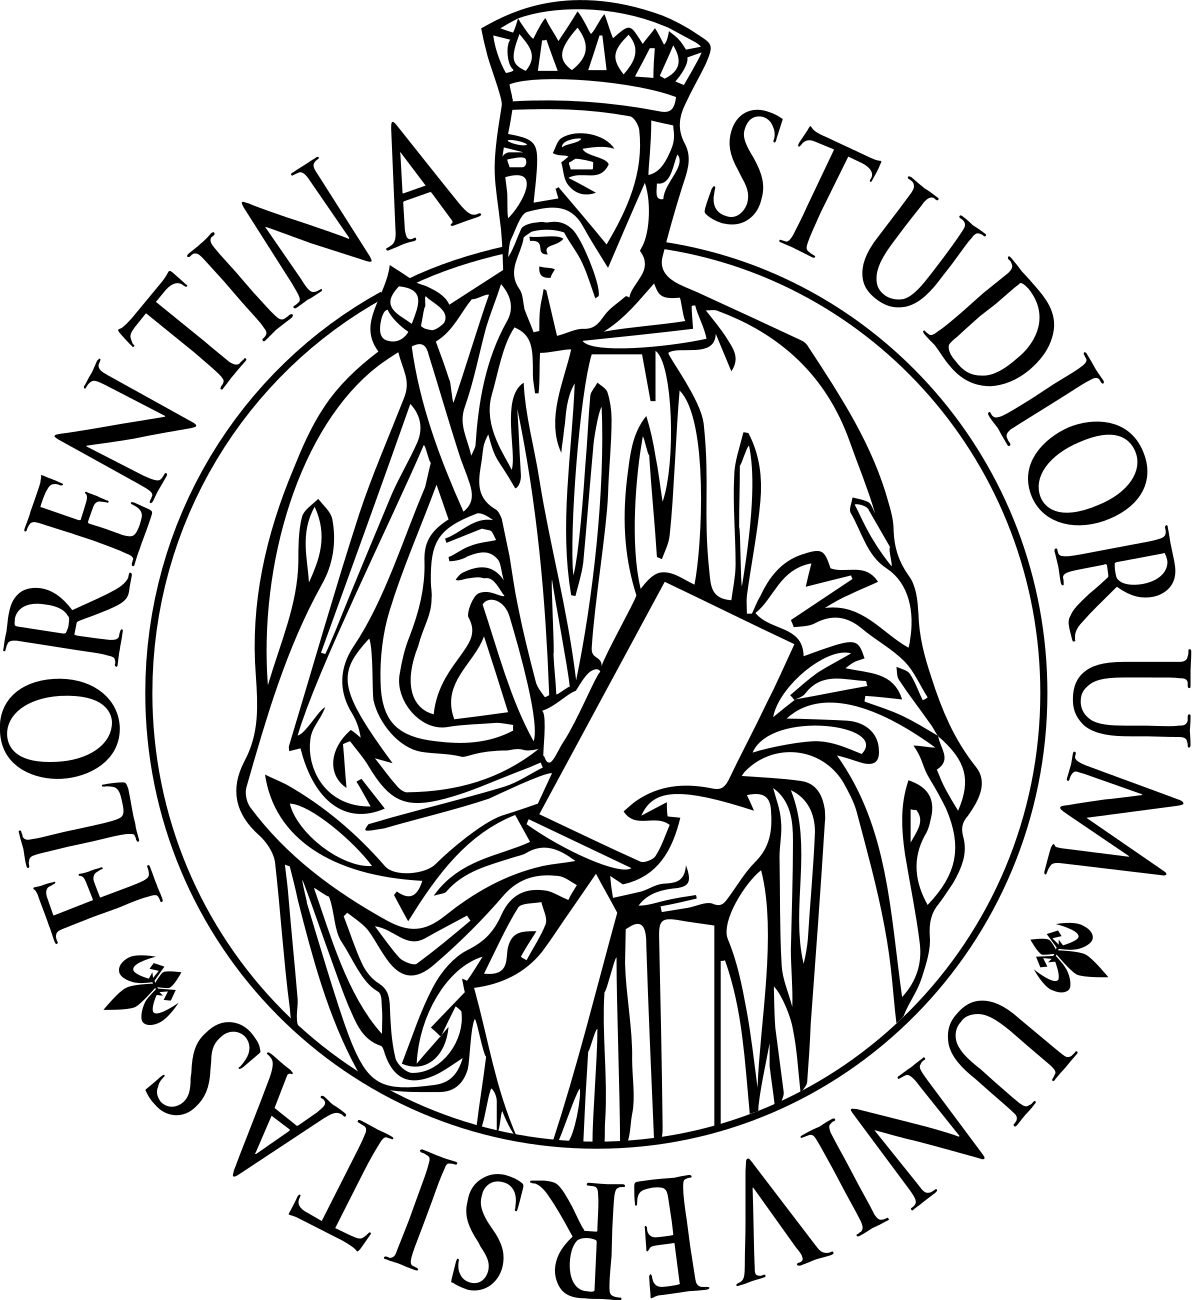
\includegraphics[width=4cm, height=4cm]{"Immagini/LogoUnifi.PNG"}
\end{figure}

\begin{center}
\textbf{\large UNIVERSITA' DEGLI STUDI DI FIRENZE \\
Facolta di Ingegneria \\
\normalsize Corso di Laurea in Ingegneria Informatica}
\end{center}

\vspace{\stretch{1}}

\newpage

% Indice
\tableofcontents

\newpage

\section{Motivazione e Descrizione}
L'idea di questo elaborato nasce da uno di noi che lavorando in una pizzeria come cameriere si è trovato ad interagire con uno di questi applicativi. Abbiamo cos\'i pensato di poterne riprodurre uno personalizzato che preveda inoltre, considerato il periodo particolare che stiamo vivendo, la possibilità di gestire azioni atte alla sicurezza dei clienti come il loro monitoraggio per poterli rintracciare. \\
L'applicativo ha lo scopo di gestire le varie parti che compongono un ristorante, in modo da farle interagire e collaborare assieme. Per il nostro applicativo abbiamo individuato cinque figure professionali principali che possono trovarsi ad agire all'interno di un ristorante:

\begin{enumerate}
\item L'organizzatore della sala è colui che all'arrivo di nuovi clienti ha il compito di assegnare loro un tavolo. Ci\'o pu\'o essere realizzato utilizzando i tavoli singoli gi\'a disposti in sala ad inizio serata o aggregandone alcuni se il numero di clienti \'e  elevato. Ha quindi la possibilit\'a di contrassegnare i tavoli assegnati come occupati e di rimetterli disponibili una volta terminato il servizio e igenizzato il tavolo. Inoltre, in vista delle norme di distanziamento imposte dal periodo che stiamo vivendo, l'organizzatore della sala pu\'o decidere se e quali tavoli sono o no utilizzabili. 
\item Il cameriere ha il compito di gestire i vari servizi ai tavoli, ossia di prendere le comande e mandarle alla cucina per la loro realizzazione. Le comande si compongono da un insieme di piatti presenti nel men\'u del locale, da dei commenti opzionali sui piatti per la cucina e da un insieme di ingredienti aggiunti/rimossi dalle varie portate su preferenza e richiesta del cliente. In caso di  errore di immissione della comanda o di richiesta di modifica da parte del cliente, il cameriere pu\'o eliminare le portate sbagliate in modo da correggere correttamente il conto. Per aprire un servizio al tavolo il cameriere \'e tenuto a prendere un nominativo ed un recapito telfonico di uno dei presenti in modo da tenerne traccia di chi ha frequentato il locale ed essere in grado di rintracciare i clienti in caso di necessit\'a. 
\item La cucina e quindi i cuochi ottengono le comande confermate dai camerieri ai vari tavoli e, una volta preparate, possono spuntarle come gi\'a fatte. La cucina si pu\'o inoltre specializzare in pi\'u aree di competenza come ad esempio la pizzeria e il bar. 
\item Il cassiere \'e colui che al termine del servizo a un tavolo esegue il conto, contrassegna il tavolo come da pulire ed igenizzare e si occupa di memorizzare correttamente i dati dei clienti presenti.
\item Il gestore del ristorante \'e colui che ha accesso ai dati memorizzati dei clienti. Pu\'o inoltre modificare il men\'u del locale aggiungendo portate e variando gli ingredienti in esse presenti al fine per esempio di aggiungere una specialit\'a del giorno.
\end{enumerate}

\subsection{Possibili aggiunte}

Delle possibili aggiunte non implementate potrebbero essere quelle di consentire al cliete di fare degli ordini da casa attraverso un sistema di consegna a domicilio (Es: Delivero) oppure quella di consenire all'organizzatore della sala di poter gestire le prenotazioni future dei clienti attraverso app. Login dei vari dipendenti. 

% Insieme

\section{Requisiti}
\subsection{Use Case}
Dalla descrizione del nostro modello di dominio, abbiamo individuato nelle varie figure professionali del ristorante gli attori in gioco e nelle loro mansioni i corrispettivi casi d'uso. Riportiamo quindi di seguito l'Use Case Diagram risultante:

\begin{figure}[!h]
\centering
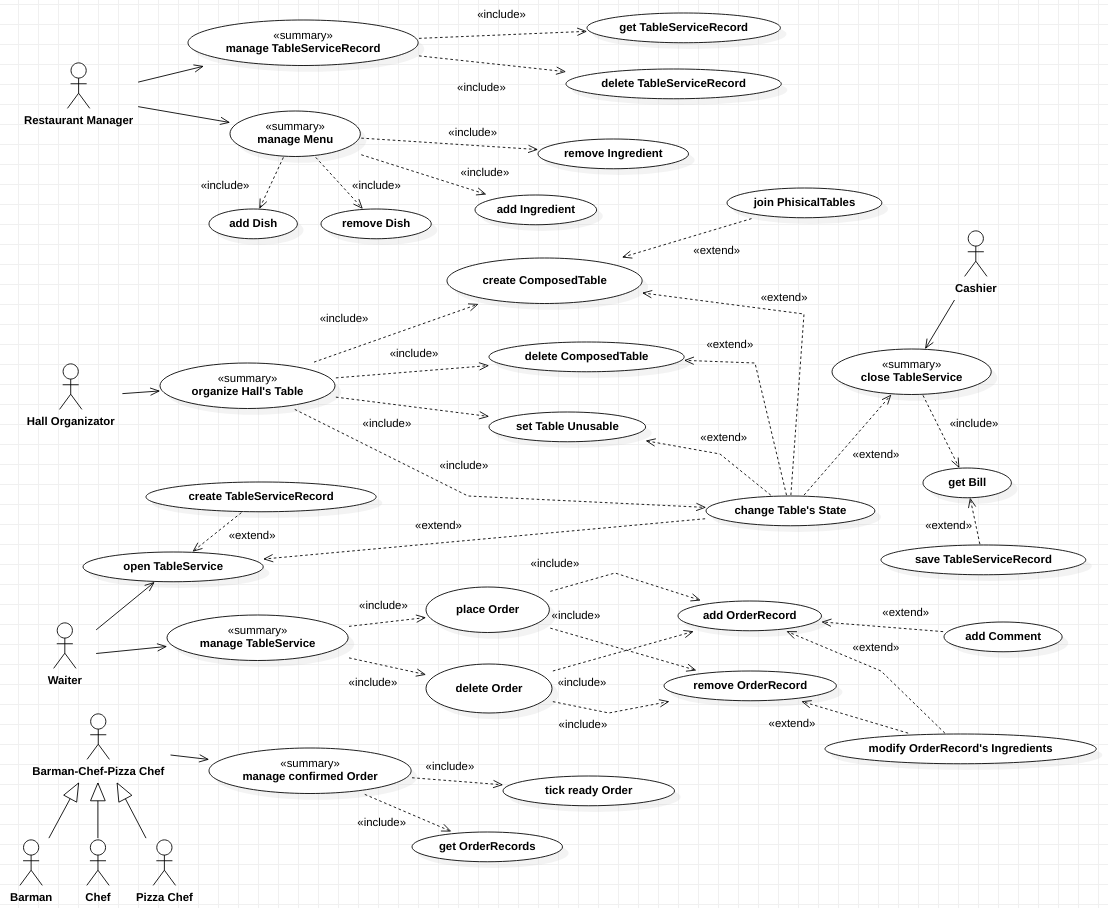
\includegraphics[width= 15cm, height= 11cm]{"Immagini/UseCaseDiagram.PNG"}
\caption{Use Case Diagram}
\end{figure}

\newpage

\subsection{Use Case Template}
Riportiamo di seguito dei template relativi ad alcuni dei pricipali casi d'uso individuati nel nostro progetto:

% betta

\subsection{Mockups}
Riportiamo di seguito dei possibili mockups relativi alle interfaccie grafiche della nostra app per l'interazione con i nostri attori.

\begin{figure}[!h]
\centering
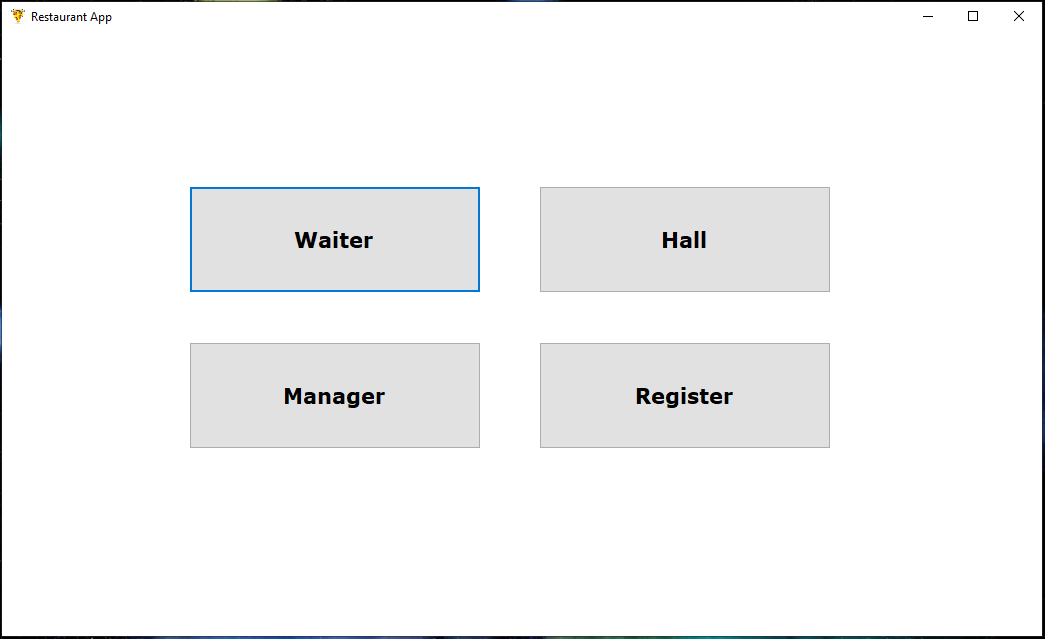
\includegraphics[width= 10cm, height= 6cm]{"Immagini/HomePage.PNG"}
\caption{Mockup raffigurante un prototipo della home page dell'app}
\end{figure}

\begin{figure}[!h]
\centering
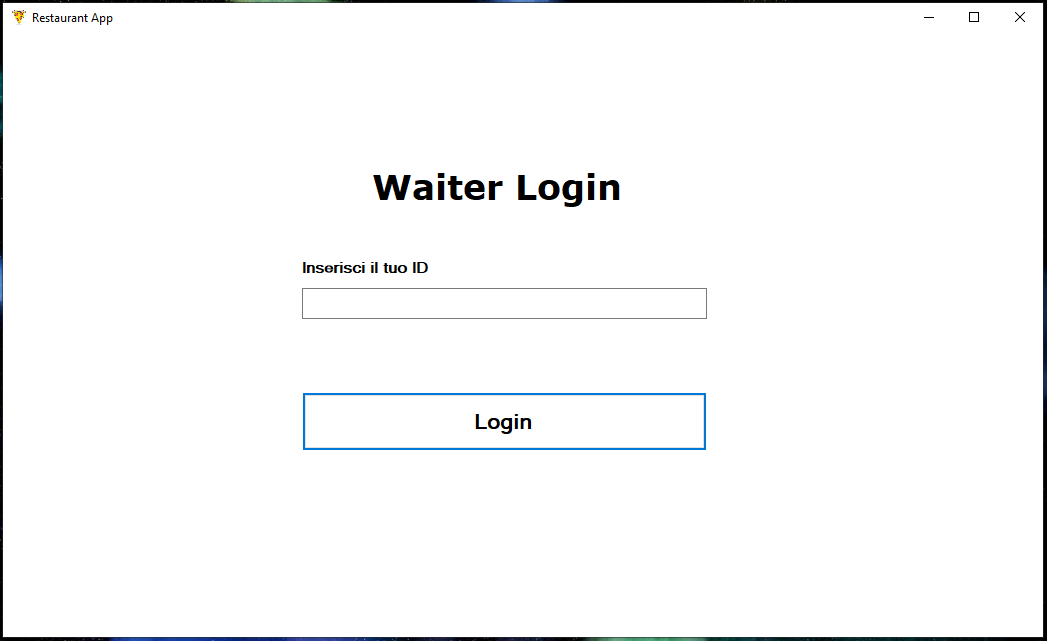
\includegraphics[width= 10cm, height= 6cm]{"Immagini/WaiterLogin.PNG"}
\caption{Mockup raffigurante un prototipo della pagina di login del cameriere}
\end{figure}

\begin{figure}[!h]
\centering
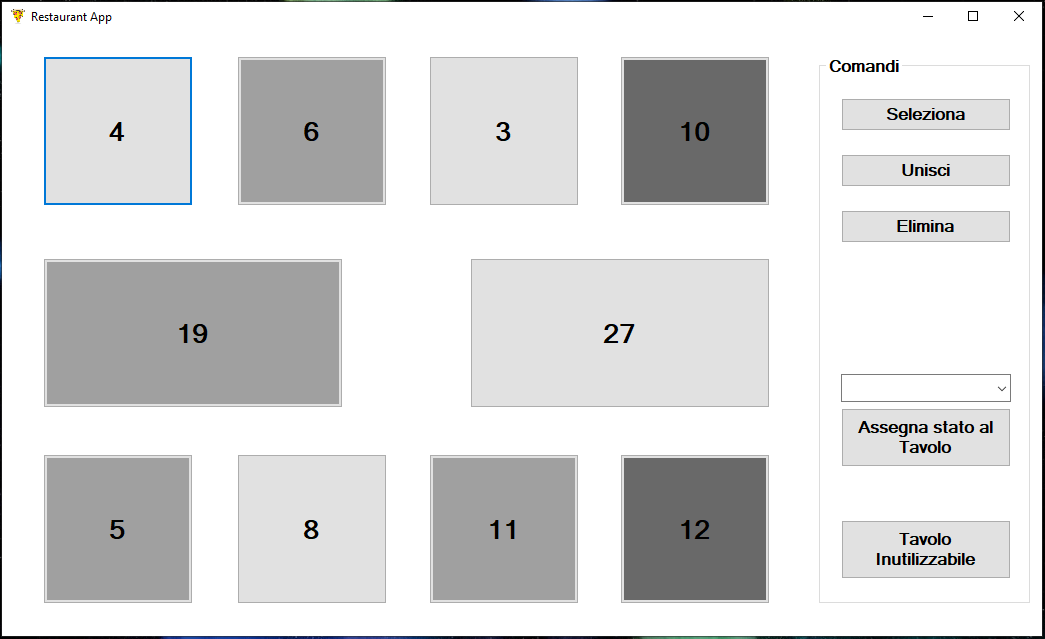
\includegraphics[width= 10cm, height= 6cm]{"Immagini/HallOrganizatorPage.PNG"}
\caption{Mockup raffigurante un prototipo dell'interfaccia dell'organizzatore della sala}
\end{figure}

\begin{figure}[!h]
\centering
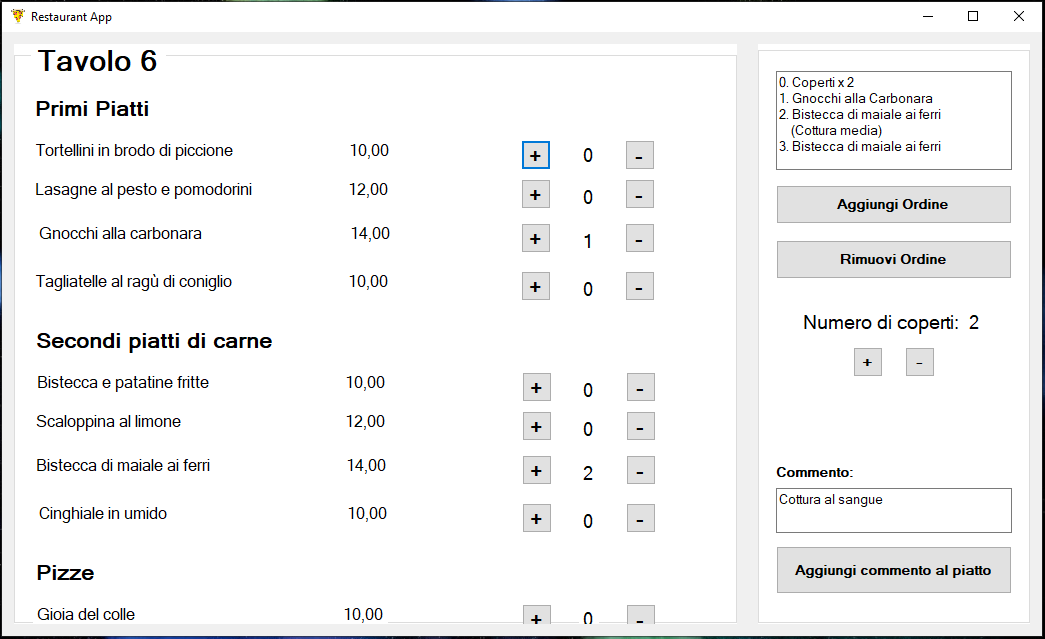
\includegraphics[width= 10cm, height= 6cm]{"Immagini/OrdineCameriere.PNG"}
\caption{Mockup raffigurante un prototipo dell'interfaccia del cameriere al momento della creazione di un ordine}
\end{figure}

\section{Progettazione e Implementazione}
\subsection{Scelte implementative e considerazioni}
L'applicativo si presta per essere relalizzato ed opearare come un sistema distribuito, prevedendo cio\'e un server centrale con al suo interno i dati comuni accessibili dai vari terminali attraverso un protocollo di comunicazione. Per le competenze richieste dall'elaborato, lo schema da noi riportato e implementato ha il solo scopo di illustrare le interazioni principali fra le varie parti, non \'e quindi atto ad una realizzazione concreta.  

% insieme

\subsection{Class Diagram}
Qui di seguito riportiamo la realizzazione del Class Diagram che descrive la nostra logica di dominio in prospettiva di implementazione:

\begin{figure}[!h]
\centering
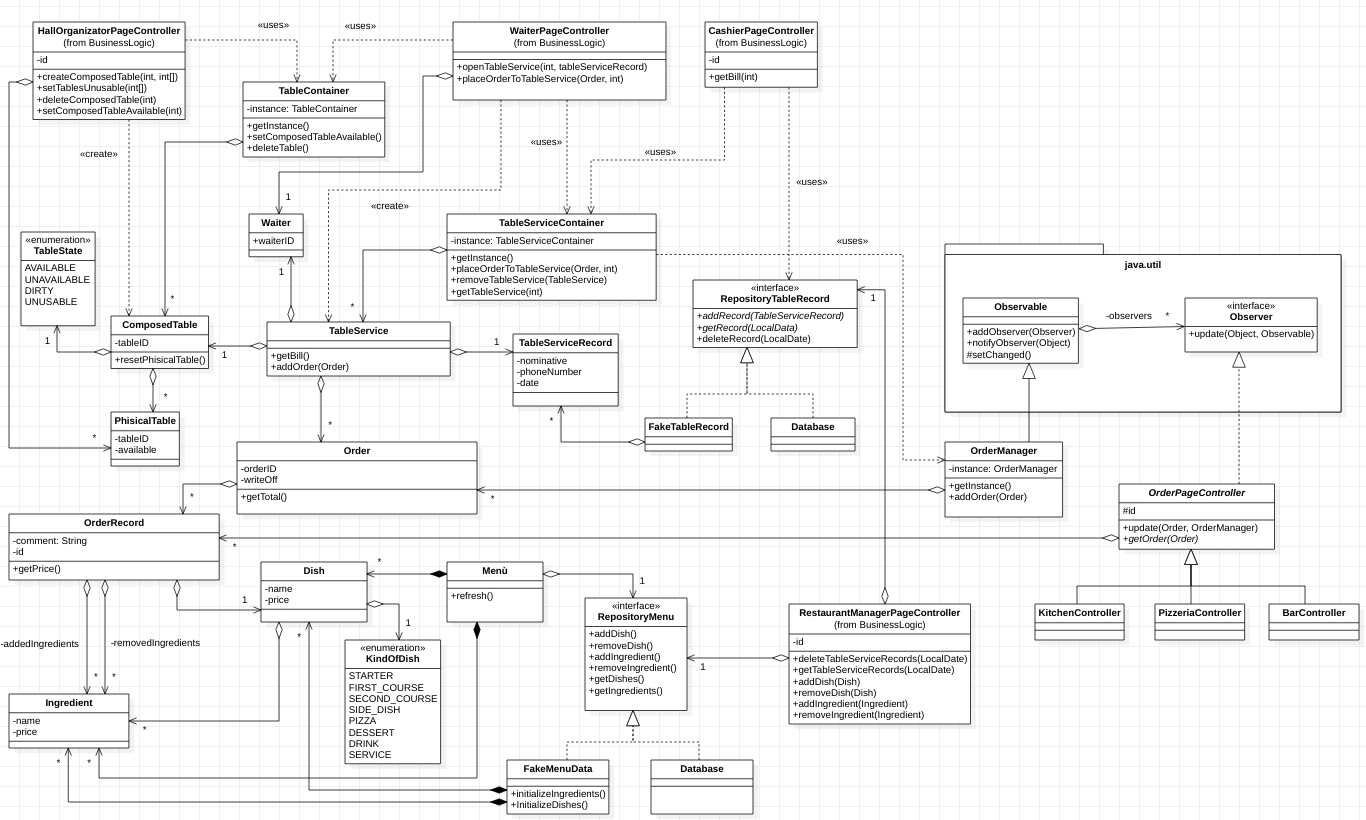
\includegraphics[width= 15cm, height= 11cm]{"Immagini/ClassDiagram.PNG"}
\caption{Class Diagram}
\label{ClassDiagram}
\end{figure}

\newpage

\subsection{Classi ed Interfacce}
Per l'implementazione del nostro applicativo abbiamo sia definito nuove classi ed interfacce specifiche per il nostro progetto, sia utilizzato alcune di quelle gi\'a presenti nelle librerie standard di Java. Le principali classi contenute nel package ... 

% gianni

\subsection{Design Patterns}
Nella realizzazione del nostro progetto ci siamo imbattuti in delle situazioni dove \'e emersa la necessit\'a di introdurre dei design patterns noti al fine di gestirle in modo agile ed elegante. I patterns utilizzati nel nostro applicativo sono: 

\begin{enumerate}
\item Observer
\item Singleton
\item MVC
\end{enumerate}

\subsubsection{Observer}

Il pattern Comportamentale Observer \'e utilizzato per notificare ad uno o pi\'u oggetti che svolgono il ruolo di osservatori quando un altro elemento osservato varia il suo stato di interesse. \\
Nella nostra logica di dominio abbiamo avuto la necessit\'a di introdurre questo pattern per notificare alla cucina l'invio da parte del cameriere di una nuova comanda presa a un tavolo. Nonostante siano state deprecate, per implementare il pattern Observer ci siamo serviti delle classi "Observable" e "Observer" e dei loro rispettivi metodi "notify" e "update" forniti dalla libreria java.util. Abbiamo inoltre deciso di implementare il pattern Observer in modalit\'a push, la quale prevede che l'oggetto osservato notifichi gli osservatori inviando direttamente il cambiamento al momento della sua variazione. \\ Come \'e possibile infatti apprezzare dal Class Diagram di Figura \ref{ClassDiagram}, la classe Order Manager svolge il ruolo di oggetto osservato (Observable) che notifica l'arrivo di una nuova comanda inviandola direttamente alla cucina, alla pizzeria e al bar che svolgono il ruolo di osservatori (Observer). Questo avviene attraverso il metodo "addOrder" che preso come parametro il nuovo ordine piazzato dal cameriere lo invia agli Observers attraverso il metodo "notify", questi ultimi aggiorneranno poi il loro stato attraverso il metodo "update" (Vedi Sequence Diagram in Figura \ref{SequenceDiagram}).

\newpage

\subsubsection{Singleton}

Il pattern Creazionale Singleton \'e utilizzato per avere un'unica istanza di una determinata classe. \\
Nel nostro progetto abbiamo infatti introdotto questo pattern per garantire l'unicit\'a delle istanze delle classi "TableContainer", "TableServiceContainer" e "OrderManager", le quali interagiscono con pi\'u attori e classi e si ha quindi la necessit\'a che siano sempre le stesse. Come \'e possibile osservare nel Sequence Diagram di Figura \ref{SequenceDiagram}, gli attori non possiedono i riferimenti a l'unica instanza di queste classi, ma li ottengono al momento che necessitano di utilizzarle attraverso il rispettivo metodo "getInstance".

\subsubsection{MVC}

Il pattern Architetturale Model-View-Controller \'e utilizzato quando si ha la necessit\'a di accedere e modificare dei dati attraverso interazioni differenti con i client. Per far questo si possono dunque individuare le tre componenti principali:

\begin{itemize}
\item Model: \'E la parte che definisce il modello dei dati e le operazioni che possono essere  eseguite su queste presentandole alla View e al Controller. Il Model pu\'o inoltre notificare ai vari componenti della View eventuali aggiornamenti in seguito a richieste del Controller al fine di presentare ai Client dati sempre aggiornati.

\item View: Corrisponde alle varie interfacce dell'applicazione con cui gli utenti si possono trovare ad interagire per eseguire delle azioni sul sistema.
 
\item Controller: Svolge il ruolo da mediatore fra il View e il Model, trasformando le interazioni dell'utente sul primo in azioni sul secondo. Per farlo sfrutta inoltre un meccanismo che prende il nome di business logic. Questo consiste nel mettere in vita determinati oggetti del Model solo nel momento del loro effettivo bisogno ossia quando devono interagire in risposta alle richieste del client.
\end{itemize}

\newpage

Riportiamo di seguito l'architettura del nostro applicativo suddivisa nelle tre componenti sopra descritte:

\begin{figure}[!h]
\centering
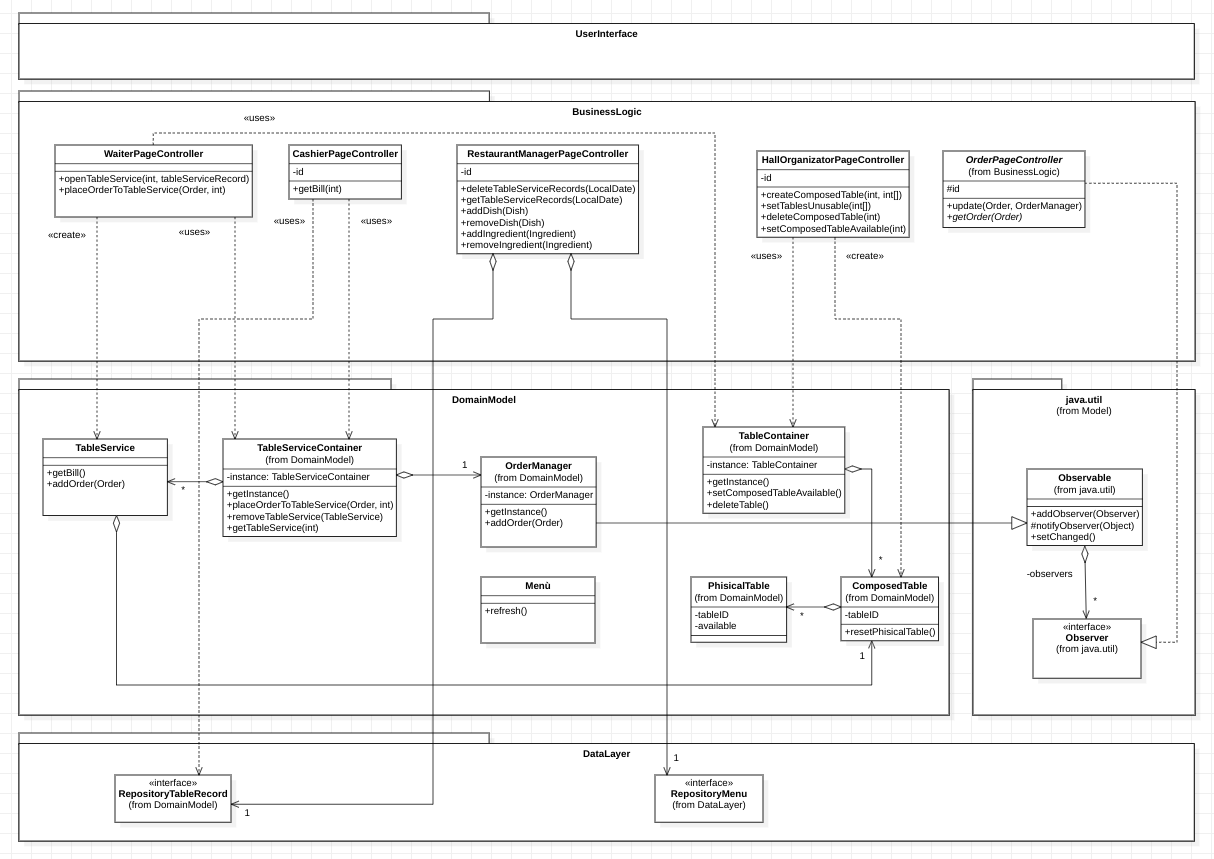
\includegraphics[width= 14cm, height= 12cm]{"Immagini/Architecture.PNG"}
\caption{Raffigurazione dell'architettura dell'applicativo secondo lo schema Model-View-Controller}
\end{figure}

\newpage

\subsection{Disposizione delle classi nei package} 

\begin{figure}[!h]
\centering
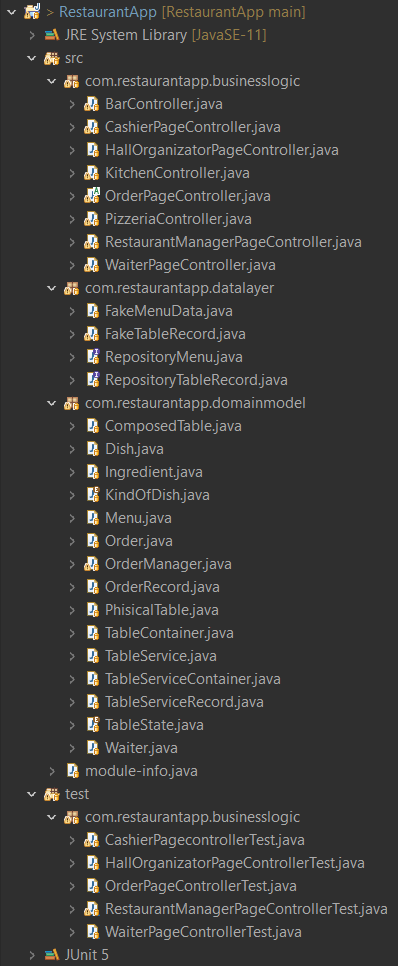
\includegraphics[width= 6cm, height= 11cm]{"Immagini/Package.PNG"}
\caption{Raffigurazione della disposizione delle classi del progetto nei package}
\end{figure}

\section{UnitTest e flusso di controllo}
\subsection{Unit Test}
Per testare la corretta interazione e collabborazione fra le parti abbiamo deciso di eseguire i seguenti test sui principali casi d'uso dei nostri attori...

% betta

\newpage

\subsection{Sequence Diagram}
Di seguito riportiamo un possibile scenario di interazione dei nostri attori:

\begin{figure}[!h]
\centering
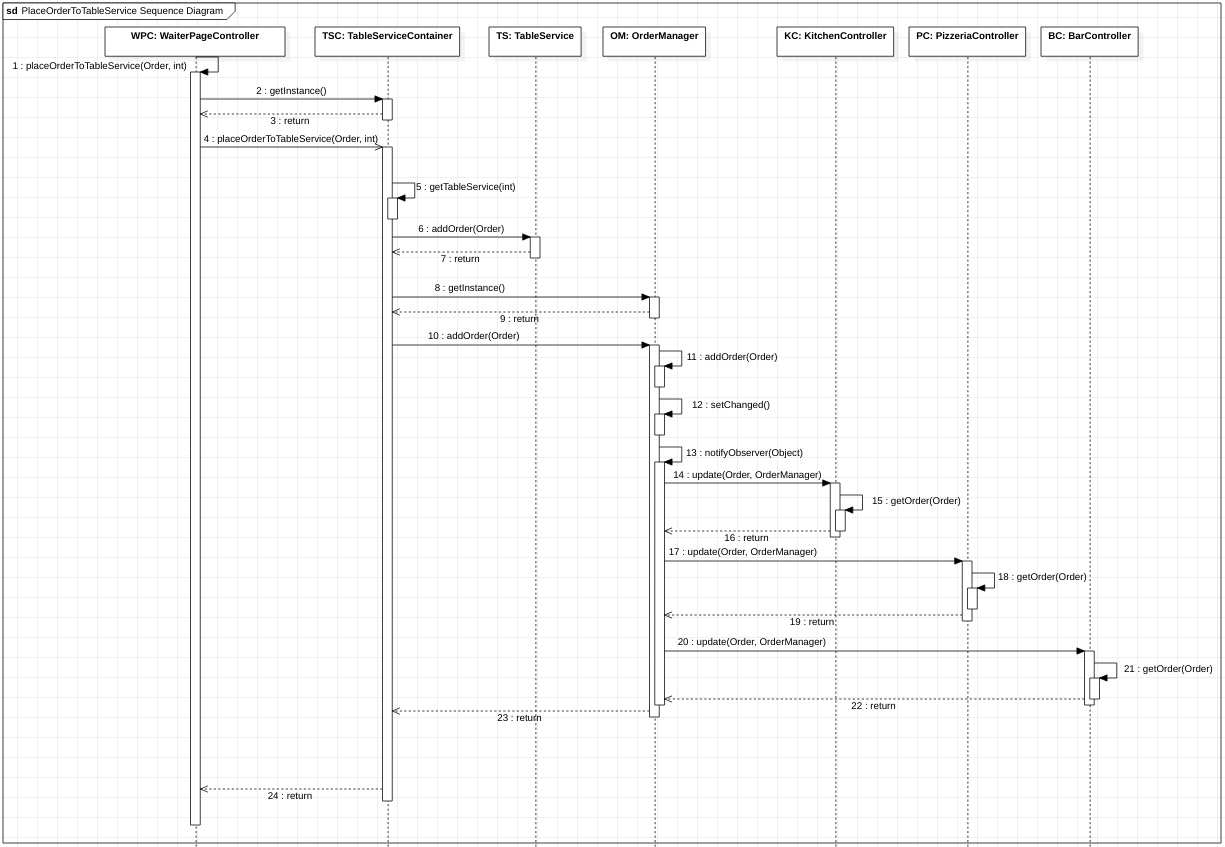
\includegraphics[width= 15cm, height= 12cm]{"Immagini/SequenceDiagram.PNG"}
\caption{Sequence Diagram che documenta il flusso del controllo nel momento in cui il cameriere piazza un nuovo ordine a un tavolo}
\label{SequenceDiagram}
\end{figure}

\end{document}